%!TEX root = main.tex

\section{Overviews of The Methodology}
\seclabel{overview}
%
%
\JW{Fixed: In general, I think this section needs to describe the ACC example (which it does) but also needs to make sure the reviewers know how everything can be generalized.  These insights will segue nicely to the \toolreaffirm discussion in the next section.}
%
In this section, we will explain our methodology through a toy example of an adaptive cruise control system (ACC). This system has been designed to satisfy safety requirements pertaining to vehicle spacing that varies with vehicle speed.
%which aims to safely adapt a vehicle speed
%In the following, we first present the original (legacy) system which satisfies an initial functional safety requirement. 
%
Assume that a designer has previously modeled the ACC system as a combination of the vehicle dynamics and an control module, and resiliency was not considered in the initial design. In the following, we will describe the ACC system as originally designed, its attack scenario, and an example of resiliency pattern to repair the ACC model\footnote{We note that the ACC model presented herein is not a representative of the complexity of a true ACC system, but a toy example in which the dynamics and control equations are chosen for simplicity in the ensuing discussion of the paper.}.
%
Then, we present the structure of \toolreaffirm and demonstrate how \toolreaffirm can automatically perform a model transformation and synthesis to construct a new ACC model with resiliency. 
%
%which will (in the subsequent discussion) be adapted to satisfy a resiliency requirement.
%
%

\subsection{Original ACC Model}
\begin{figure}[t!]%
	\centering%
	\begin{adjustbox}{max size={0.99\columnwidth}{0.75\textheight}}%
	\begin{tikzpicture}[>=stealth',shorten >=1pt,auto,node distance=8cm,font=\Large]
		%\tikzstyle{every state}=[minimum size=3cm,font=\normalsize]
		\tikzstyle{every state}=[font=\Large,rectangle,rounded corners, minimum size=5cm]
		\node[state] (speed)      			{\makecell[c]{$\textbf{Speed Control}$\\\\
		$\begin{aligned}
		\dot{d} & = \vlead - v \nonumber \\
		\dot{v} & = 2\vlead - v - \hat{v} \nonumber \\
		\dot{\hat{d}} & = \vlead - \hat{v} + 10(\drad-\hat{d})\nonumber \\
		\dot{\hat{v}} & = 2\vlead - 3\hat{v} + \frac{1}{2} (\ngps + \nenc) \nonumber\\
		\end{aligned}$\\\\
		$\hat{d} \geq 10 + 2\hat{v}$
		}};
		\node[state] (space) [right of=speed]	{\makecell[c]{$\textbf{Spacing Control}$\\\\
		$\begin{aligned}
		\dot{d} & = \vlead - v \nonumber \\
		\dot{v} & = 2\vlead - v - \hat{v} -\frac{1}{4}(10 + 2\hat{v}-\hat{d}) \nonumber \\
		\dot{\hat{d}} & = \vlead - \hat{v} + 10 (\drad-\hat{d})\nonumber \\
		\dot{\hat{v}} & = 2\vlead - 3\hat{v} + \frac{1}{2} (\ngps + \nenc) -\frac{1}{4}(10 + 2\hat{v}-\hat{d}) \nonumber\\
		\end{aligned}$\\\\
		$\hat{d} < 10 + 2\hat{v}$
		}};
		
		\node (speedtospace) [above=6mm of speed,xshift=40mm]{\makecell[c]{$\hat{d} < 10 + 2\hat{v}$}};
		%$\dot{d} = \vlead - v$\\$\dot{v} = 2\vlead - v - \hat{v} -\frac{1}{4}(10 + 2\hat{v}-\hat{d}$\\$\dot{\hat{d}} = \vlead - \hat{v} + 10(\drad-\hat{d})$\\$\dot{\hat{v}} = 2\vlead - 3\hat{v} + \frac{1}{2} (\ngps + \nenc) -\frac{1}{4}(10 + 2\hat{v}-\hat{d}$}}; 
		
		\node[coordinate] (c1) [above=5mm of speed.north] {};
		\node[coordinate] (c2) [above=5mm of space.north] {};
		\draw[->]			(speed.north) -- (c1) -- (c2) to (space.north);
		
		\node (spacetospeed) [below=6mm of space,xshift=-40mm]{\makecell[c]{$\hat{d} \geq 10 + 2\hat{v}$}};

		\node[coordinate] (c3) [below=5mm of space.south] {};
		\node[coordinate] (c4) [below=5mm of speed.south] {};
		\draw[->]			(space.south) -- (c3) -- (c4) to (speed.south);
		%
		%\path[->]			(speed.north) edge[bend left] node{\makecell[c]{$\mathit{OD} \leq \mathit{OD}_t \wedge t_m \geq t_\text{mOn} $\\$t_m' := 0$}} (space.north); 
		%\path[->]			(space.south)	edge[bend left] node{\makecell[c]{$\mathit{OD} \geq \mathit{OD}_t \wedge t_m \geq t_\text{mOff} $\\$t_m' := 0$}} (speed.south); 
	\end{tikzpicture}%
	\end{adjustbox}%
	\caption{Original ACC model}%
	\figlabel{original}%
\end{figure}

%To illustrate and motivate our proposed approach, this subsection presents a case study of a control system that aims to safely adapt a vehicle speed, namely, an adaptive cruise control (ACC) system. 

%
%\noindent
%{\bf Original ACC Model.}
\JW{Fixed: I think we need to acknowledge -- possibly within the subsection title -- that this is a toy example.  Reviewers may take issue with our work if they think that we believe the ACC model used herein is representative of the complexity of a true ACC system.}
%
The original ACC system operates in two modes: \emph{speed control} and \emph{spacing control}. In speed control, the host car travels at a driver-set speed. In spacing control, the host car aims to maintain a safe distance from the lead car. 
%
The ACC system decides which mode to use based on the real-time sensor measurements. 
%
For example, if the lead car is too close, the ACC system switches from speed control to spacing control. 
%
Similarly, if the lead car is further away, the ACC system switches from spacing control to speed control. %In other words, the ACC system makes the host car travel at a driver-set speed as long as a safe distance is maintained.
%
The vehicle has two states in which $d$ is the distance to the lead car, and $v$ is the speed of the host vehicle. These states evolve according to $\dot{d} = \vlead - v$ and $\dot{v} = -v + u$, \JW{Fixed: Again, I think we need to be absolutely honest that these equations are chosen to simplicity in the ensuing discussion.}
%
where $\vlead$ is the speed of the lead vehicle  and $u$ is the control input.  In this example, we assume that the lead vehicle speed is known exactly (\eg it is communicated between vehicles). Conceptually, the dynamics for $d$ represent that the derivative of the relative distance is the difference between the lead vehicle speed and the host vehicle speed. The dynamics for the host vehicle speed indicate that as the vehicle speed increases, it takes more acceleration (\ie force) provided by the controller (\ie engine) to maintain speed. 

An ACC equipped vehicle has sensors that measure its velocity $v$ via noisy wheel encoders, $\venc = v + \nenc$, and a noisy GPS sensor, $\vgps = v+\ngps$, where $\nenc$ and $\ngps$ denote the encoder and GPS noisy, respectively. 
%
%
Additionally, the ACC system has a radar sensor that measures the distance to a (potential) lead vehicle, $\drad = d+\nrad$. 
%
To design a control law, we need to estimate the state of the vehicle (\ie we need an estimate of $d$ and $v$, which we call $\hat{d}$ and $\hat{v}$). To estimate the distance and velocity, we employ state estimators
%
\begin{align}
\dot{d} & = \vlead - \hat{v} + 10(\drad - \hat{d}) \nonumber \\
\dot{v} & = -\hat{v} + u +  (\frac{1}{2} (\vgps + \venc) - \hat{v}) 
\end{align}
%
%
\JW{Fixed: I believe the $\frac{1}{2}$ should only apply to $\vgps + \venc$ ... in other words: $\dot{v}  = -\hat{v} + u +  (  \frac{1}{2}(\vgps + \venc) - \hat{v}) $}
To implement a controller, a control law based on the state estimates in speed and distance control modes are given: 

\begin{align}
u_s & = \vlead - (\hat{v}-\vlead) \nonumber \\
u_d & = \vlead - (\hat{v}-\vlead) - \frac{1}{4} (d_{ref} - \hat{d}) 
\end{align}
%
%
where $u_s$ is the control law in the speed mode, $u_d$ is the control law in the spacing mode, and $d_{ref} = 10 + 2\hat{v}$. %These control laws incorporate a reference velocity $\vlead$, which can be thought of as constant gain that depends on the lead (or desired) vehicle velocity, while the other terms depend on the deviation of the lead vehicle and and ego vehicle states.
%
%Switching between modes is handled by monitoring the state estimates. 
The designer models the complete ACC system (including vehicle dynamics) as a hybrid system, illustrated in \figref{original}. Here, the transition from speed control to spacing control occurs when the estimate of the distance is less than twice the estimated safe distance, \ie $\hat{d} < 10 + 2\hat{v}$. A similar condition is provided for transitioning from spacing control to speed control, \ie $\hat{d} \geq 10 + 2\hat{v}$. 
%
\JW{Fixed: This subsection needs to be short (like it is) but it also needs to let the reviewers know that we agree the model is simple.  Please take another attempt at it -- then I will do a pass to appease people that know something about real-world CPS modeling.}
%
%
 %Next we add a new resilience requirement that is determined to be violated by the original system. Finally, we adapt the original system such that the resilience requirement is satisfied.

\subsection{Safety Violation under GPS Sensor Attack}
%\noindent
%{\bf Attack Scenarios.}
%
In this example, the functional safety specification of the ACC system is specified that $d$ should always be greater than $d_{safe} = 5 + v$. Assume that the designer has verified the ACC system safety requirement under the scenario when $d(0) \geq 20$, $v(0) \leq 30$, $|d(0) - \hat{d}(0)| \leq 1$, $|v(0) - \hat{v}(0)| \leq 1$ , $\vlead \geq 0$, $|\nenc| \leq 0.05$ and $|\ngps| \leq 0.05$.
%
After designing the initial ACC system, it is determined that the GPS sensor can be \emph{spoofed} \cite{tippenhauer2011requirements, kerns2014unmanned}. GPS spoofing occurs when incorrect GPS packets (possibly sent by a malicious attacker) are received by the GPS receiver. In the ACC system, this allows an attacker to arbitrarily change the GPS velocity measurement. 
%
Thus, a new scenario occurs when the assumption that $|\ngps| \leq 0.05$ is omitted, and the new assumption is $|\ngps| \leq \infty$.
As a result, the safety specification could be violated under the GPS sensor attacks, and a designer needs to repair the original model with a resiliency pattern. 

\subsection{Example of Resiliency Pattern}
%
%
To provide resilience against the GPS attacks, a potential strategy is to ignore the GPS value in resilient modes and use only the wheel encoders to estimate velocity. Since the ACC system has redundancy in the sensory information of its estimated velocity, the model synthesizer can repair the model by replacing the GPS velocity measurement with the wheel encoder velocity measurement when the GPS measurement significantly deviates from the wheel encoder measurement.
%
%
Thus, the proposed fix then is first to create a resilient copy of the original model where the controller simply ignores the GPS reading as it can no longer be trusted. Then, adding new transitions from the legacy speed and spacing modes of the original model to the new resilient speed and spacing modes of the copy that uses only the wheel encoder as a velocity measurement source. We note that this transformation is generic, that is, it can be applied in a uniform manner to any given model simply by creating a duplicate version of each original mode and transition, copying the dynamics in each mode, but without a reference to the variable $\ngps$. 

%
%
\begin{figure}[!t]%frame=none,
\begin{lstlisting}[basicstyle=\ttfamily\footnotesize, numbers=none]
model = getModelByName("ACC") # retrieve the ACC model
model_copy = copyModel(model) # make a model copy 
	
# start a transformation  
addParam(model,"theta") # add new parameter theta
	
formode m = model.Mode {
		m_copy = addState(model,m)
		replace(m_copy.flow,"ngps","nenc")
		addTransition(model,m,m_copy,"abs(ngps-nenc)>theta")
}

fortran t = model_copy.Trans {
		# get source and destination modes of transition t
		src = t.source	
		dst = t.destination 
		# retrieve copies of source and destination modes 
		src_copy = getCopyState(model,src)  
		dst_copy = getCopyState(model,dst) 
		addTransition(model,src_copy,dst_copy,t.guard)
}
# end of the transformation
\end{lstlisting}
\caption{An example of a resiliency pattern written as a HATL script for the ACC system.}%
\figlabel{examplecode}%
	%\vspace{-0.5em}%
\end{figure}
%
%


~\figref{examplecode} shows an example of a resiliency pattern written as a transformation script that specifies a transformation from the original ACC model shown in~\figref{original} to the parametrized model that enables resilience. 
%
In this script, we first create a copy of the original model. Next, we iterate over each mode of the model by calling the \emph{formode loop}, make a copy with replacing the variable $\ngps$ by $\nenc$, and then add a new transition from the original mode to the copied mode with a new guard condition. This guard condition is a constraint specified over the difference between $\ngps$ by $\nenc$ and a new parameter $\theta$, which is added into the model using a function call \emph{addParam}.
%
%
Observe that while it would be possible to use only the wheel encoder all the time, a better velocity estimate must be obtained by using an average velocity measurement (from both the GPS and wheel encoders) when the GPS sensor is performing within nominal specifications. The main analysis question is when should the model switch from original copy to this resilient copy.  In this example, we model this switching condition as $|\ngps -\nenc| \geq \theta$, where $\theta$ is an unknown parameter. 



\subsection{REAFFIRM Toolkit}
%
Our \toolreaffirm prototype for the model-based design and repair with resiliency is built in Matlab and consists of main modules, corresponding to a \emph{model transformation} and a \emph{model synthesizer} as shown in \figref{overview}, and can be further interpreted as follows.
%
\begin{itemize}[leftmargin= 2 em]
    \item \textbf{Model Transformation} takes a given initial model and a resiliency pattern and generates a partial model that contains \emph{holes}, that is, parameters for which values need to be determined to ensure that the correctness requirements are satisfied. The resiliency pattern captures a generic way of transforming models that corresponds to commonly known mitigation strategies. The parameters in the incomplete model correspond to unknown switching conditions, or unknown assignments in variable updates, or even unknown coefficients in controller dynamics. The model is specified using the MathWorks Simulink/Stateflow (SLSF) format, and the correctness requirement is specified in the temporal logic Signal Temporal Logic (STL) that is widely used in tools for verification for cyber-physical systems~\cite{maler2004monitoring}. The resiliency pattern can be specified as a \emph{model transformation script} that operates on the internal representation of SLSF models specifying the desired transformation in a generic way. As an example, for a system that contains a nominal controller and a safety controller, a resiliency pattern can be specified as a transition from a nominal controller to a safety controller.
%
\item \textbf{Model Synthesizer} takes a parameterized model (SLSF) and a correctness requirement (STL formula) as inputs and outputs a completed model with parameter values instantiated to satisfy the correctness requirements.  Internally, the tool utilizes an open-source model falsification tool---Breach~\cite{donze2010breach}, to check an SLSF model against the specification. The counterexamples returned by this falsification tool are used to determine values for the desired parameters. At the end of a falsification loop, the completed model produced by \toolreaffirm, compared to the partial behavior model, can have additional modes of operation as well as new transitions between different modes, and as a result, has resilient behaviors specified in the resiliency patterns.
\end{itemize}
%
%
%
%
\begin{figure}[t!]%
	\centering%
    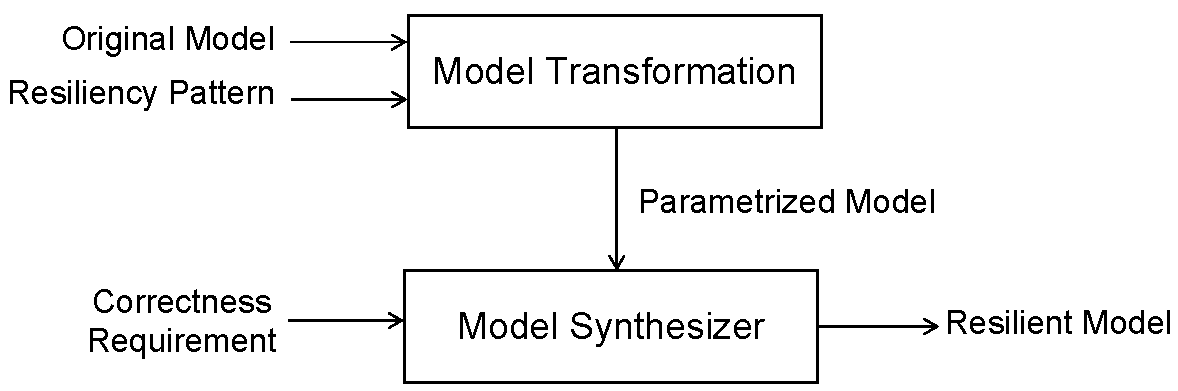
\includegraphics[width=0.48\textwidth]{image/overview}%
		%\includegraphics[trim = 17mm 85mm 17mm 0mm, clip, width=0.95\textwidth]{image/spectral_signal}%
		%\vspace{-1em}
	\caption{\toolreaffirm Overview.}%
	\figlabel{overview}%
	%\vspace{-1em}
\end{figure}%
%
%

To provide a resilience for the ACC model, the transformation tool of \toolreaffirm will take the original ACC model shown in ~\figref{original} and the transformation script demonstrated in \figref{examplecode}, and then output the \emph{parameterized} model displayed in \figref{updated}, where the variable $\ngps$ is replaced by the variable $\nenc$ in the resilient speed and spacing control modes, and the value of $\theta$ needs to be determined. Next, the model synthesizer of \toolreaffirm takes the parameterized ACC model, the safety requirement encoded as an STL formula $\Box_{[0, \infty]} (d[t] < 5 + v[t])$, and the specific range of $\theta$, and then calls the synthesizer to determine the best $\theta$ which ensures the final model will always satisfy the safety requirement. If the tool cannot find any value of $\theta$ over a given range, it will suggest a designer to either search over different parameter ranges or try different resiliency patterns.   
%
%

\begin{figure}[t!]%
	\centering%
	\begin{adjustbox}{max size={0.99\columnwidth}{0.75\textheight}}%
	\begin{tikzpicture}[>=stealth',shorten >=1pt,auto,node distance=8cm,font=\Large]
		%\tikzstyle{every state}=[minimum size=3cm,font=\normalsize]
		\tikzstyle{every state}=[font=\Large,rectangle,rounded corners, minimum size=5cm]
		\node[state] (speed)      			{\makecell[c]{$\textbf{Speed Control}$\\\\
		$\begin{aligned}
		\dot{d} & = \vlead - v \nonumber \\
		\dot{v} & = 2\vlead - v - \hat{v} \nonumber \\
		\dot{\hat{d}} & = \vlead - \hat{v} + 10(\drad-\hat{d})\nonumber \\
		\dot{\hat{v}} & = 2\vlead - 3\hat{v} + \frac{1}{2} (\ngps + \nenc) \nonumber\\
		\end{aligned}$\\\\
		$\hat{d} \geq 10 + 2\hat{v}$
		}};
		\node[state] (space) [right of=speed]	{\makecell[c]{$\textbf{Spacing Control}$\\\\
		$\begin{aligned}
		\dot{d} & = \vlead - v \nonumber \\
		\dot{v} & = 2\vlead - v - \hat{v} -\frac{1}{4}(10 + 2\hat{v}-\hat{d}) \nonumber \\
		\dot{\hat{d}} & = \vlead - \hat{v} + 10 (\drad-\hat{d})\nonumber \\
		\dot{\hat{v}} & = 2\vlead - 3\hat{v} + \frac{1}{2} (\ngps + \nenc) -\frac{1}{4}(10 + 2\hat{v}-\hat{d}) \nonumber\\
		\end{aligned}$\\\\
		$\hat{d} < 10 + 2\hat{v}$
		}};
		
		\node[state] (res_speed) [below of=speed]  {\makecell[c]{$\textbf{Resilient Speed Control}$\\\\
		$\begin{aligned}
		\dot{d} & = \vlead - v \nonumber \\
		\dot{v} & = 2\vlead - v - \hat{v} \nonumber \\
		\dot{\hat{d}} & = \vlead - \hat{v} + 10(\drad-\hat{d})\nonumber \\
		\dot{\hat{v}} & = 2\vlead - 3\hat{v} + \frac{1}{2} (\nenc + \nenc) \nonumber\\
		\end{aligned}$\\\\
		$\hat{d} \geq 10 + 2\hat{v}$
		}};
		
		\node[state] (res_space) [right of=res_speed]	{\makecell[c]{$\textbf{Resilient Spacing Control}$\\\\
		$\begin{aligned}
		\dot{d} & = \vlead - v \nonumber \\
		\dot{v} & = 2\vlead - v - \hat{v} -\frac{1}{4}(10 + 2\hat{v}-\hat{d}) \nonumber \\
		\dot{\hat{d}} & = \vlead - \hat{v} + 10 (\drad-\hat{d})\nonumber \\
		\dot{\hat{v}} & = 2\vlead - 3\hat{v} + \frac{1}{2} (\nenc + \nenc) -\frac{1}{4}(10 + 2\hat{v}-\hat{d}) \nonumber\\
		\end{aligned}$\\\\
		$\hat{d} < 10 + 2\hat{v}$
		}};
		
		
		\node (speedtospace) [above=6mm of speed,xshift=40mm]{\makecell[c]{$\hat{d} < 10 + 2\hat{v}$}};
		%$\dot{d} = \vlead - v$\\$\dot{v} = 2\vlead - v - \hat{v} -\frac{1}{4}(10 + 2\hat{v}-\hat{d}$\\$\dot{\hat{d}} = \vlead - \hat{v} + 10(\drad-\hat{d})$\\$\dot{\hat{v}} = 2\vlead - 3\hat{v} + \frac{1}{2} (\ngps + \nenc) -\frac{1}{4}(10 + 2\hat{v}-\hat{d}$}}; 
		
		\node[coordinate] (c1) [above=5mm of speed.north] {};
		\node[coordinate] (c2) [above=5mm of space.north] {};
		\draw[->]			(speed.north) -- (c1) -- (c2) to (space.north);
		
		\node (spacetospeed) [below=6mm of space,xshift=-40mm]{\makecell[c]{$\hat{d} \geq 10 + 2\hat{v}$}};

		\node[coordinate] (c3) [below=5mm of space.south] {};
		\node[coordinate] (c4) [below=5mm of speed.south] {};
		\draw[->]			(space.south) -- (c3) -- (c4) to (speed.south);
		
		\node (res_speedtospace) [above=6mm of res_speed,xshift=40mm]{\makecell[c]{$\hat{d} < 10 + 2\hat{v}$}};
		%$\dot{d} = \vlead - v$\\$\dot{v} = 2\vlead - v - \hat{v} -\frac{1}{4}(10 + 2\hat{v}-\hat{d}$\\$\dot{\hat{d}} = \vlead - \hat{v} + 10(\drad-\hat{d})$\\$\dot{\hat{v}} = 2\vlead - 3\hat{v} + \frac{1}{2} (\ngps + \nenc) -\frac{1}{4}(10 + 2\hat{v}-\hat{d}$}}; 
		
		\node[coordinate] (c5) [above=5mm of res_speed.north] {};
		\node[coordinate] (c6) [above=5mm of res_space.north] {};
		\draw[->]			(res_speed.north) -- (c5) -- (c6) to (res_space.north);
		
		\node (res_spacetospeed) [below=6mm of res_space,xshift=-40mm]{\makecell[c]{$\hat{d} \geq 10 + 2\hat{v}$}};

		\node[coordinate] (c7) [below=5mm of res_space.south] {};
		\node[coordinate] (c8) [below=5mm of res_speed.south] {};
		\draw[->]			(res_space.south) -- (c7) -- (c8) to (res_speed.south);
		
		\node[coordinate] (c9) 	[left=5mm of speed.south] {};
		\node[coordinate] (c10) [left=5mm of res_speed.north] {};
		\node[coordinate] (c11) [right=5mm of space.south] {};
		\node[coordinate] (c12) [right=5mm of res_space.north] {};
		
		%\draw[->]			(speed.south)[right=1mm to (res_speed.north);
		%\draw[->]			(space.south) to (res_space.north);
		
		\path[->]			(c9) edge node[xshift=-29mm]{\makecell[c]{$|\ngps -\nenc| \geq \theta$}}(c10); 
		\path[->]			(c11) edge node[xshift=1mm]{\makecell[c]{$|\ngps -\nenc| \geq \theta$}} (c12); 
		
		%
		%\path[->]			(speed.north) edge[bend left] node{\makecell[c]{$\mathit{OD} \leq \mathit{OD}_t \wedge t_m \geq t_\text{mOn} $\\$t_m' := 0$}} (space.north); 
		%\path[->]			(space.south)	edge[bend left] node{\makecell[c]{$\mathit{OD} \geq \mathit{OD}_t \wedge t_m \geq t_\text{mOff} $\\$t_m' := 0$}} (speed.south); 
	\end{tikzpicture}%
	\end{adjustbox}%
	\caption{Updated Resilient ACC model}%
	\figlabel{updated}%
\end{figure}

%